\documentclass[12pt]{article}
\usepackage{graphicx}
\usepackage{times}
\usepackage{draftwatermark}
\graphicspath{ {./figures/} }
\title{Prioritizing Water Quality Improvement Efforts on Agricultural Lands Using LiDAR Elevation Data}
\author{
	Aaron S. Ruesch\\
	Theresa Nelson\\
	Bureau of Water Quality\\
	Wisconsin Department of Natural Resources\\
	Aaron.Ruesch@wisconsin.gov
}
\date{\today}
\begin{document}
\maketitle
\section{Background}
On the basis of intensive inventories of farm management in southwestern Wisconsin, an estimated 63\% of phosphorus loads from agricultural runoff can be traced back to only 18\% of agricultural fields (unpublished data). That is, the majority of nutrient pollution, and the ecological and societal impacts of the associated algal blooms, is coming from a minority of farms. It follows that the majority of agricultural nutrient pollution can be reduced with fewer resources in terms of the implementation of best management practices (BMPs). However, this logic presumes that the critical source areas (CSAs) are identified correctly \cite{weld_identifying_2001}---if agricultural fields are incorrectly identified, the resulting BMPs may have little or no detectable effect on downstream water quality because the agricultural field historically contributed only a small fraction of the total pollutant load.

In the past, Wisconsin farmers voluntarily participated in water quality improvement programs \cite{wisconsin_department_of_natural_resources_wisconsins_2011} through cost-sharing grants or incentive programs such as the Conservation Reserve Program (CRP). Voluntary participation presumes that a farm is willing to change a given management practice in favor of one that improves water quality---this selection process is likely biased toward farms that are already implementing best-management practices, and thus contribute a smaller fraction of the downstream load. Therefore, voluntary programs are more likely to result in little to no detectable downstream improvement.

To acheive the greatest reduction with the fewest resources, farms must be correctly identified as CSAs. Identifying CSAs correctly has historically been a challenge for watershed managers, especially when they are interested in reducing phosphorus loads. Excluding the estimation of the delivery ratio from any given field, the phosphorus load leaving the edge of an agricultural field can be difficult to estimate \cite{nelson_evaluation_2012}. Edge-of-field estimates often rely on complex models that require an abundance of input data, such as annual tillage practices and fertilizer type/amount/timing. These data can be difficult to measure and are often protected under strict privacy constraints. Including the delivery ratio into the estimate makes estimation even more difficult due to the volume of required inputs into the model and the fact that phosphorus transport is relatively poorly understood. These limitations to estimation can create cost barriers before a project even begins the implementation phase.

To reduce the cost associated with identifying critical source areas, we have developed quantitative, push-button, software tools for prioritizing targeting efforts within a watershed. The tools are based on novel methods that were first developed by Houston Engineering, Inc. for targeting in the Red River Basin in Minnesota. However, the tools were never released to the public, and thus could not be easily replicated. The methodology is based on easily available spatial data (e.g., aerial imagery, digital elevation models) that allows a watershed manager to infer the locations of fields that are vulnerable to nutrient or sediment loss with minimal effort in terms of data collection or processing. Using a simple, cost-effective, prioritization approach to targeting reduces the need to collect watershed-wide agricultural inventories. Rather than estimating precisely the pollutant load associated with all agricultural fields, we propose a simpler method that prioritizes based on disproportionate vulnerability---a more precise estimate of load reduction based on intensive agricultural inventories can then be calculated from a subset of only the most vulnerable fields (Figure~\ref{decisionFramework}). These methods allow more efficient and effective use of local watershed management staff (e.g., counties) while also having a greater impact on water quality.

\begin{figure}
  \centering
    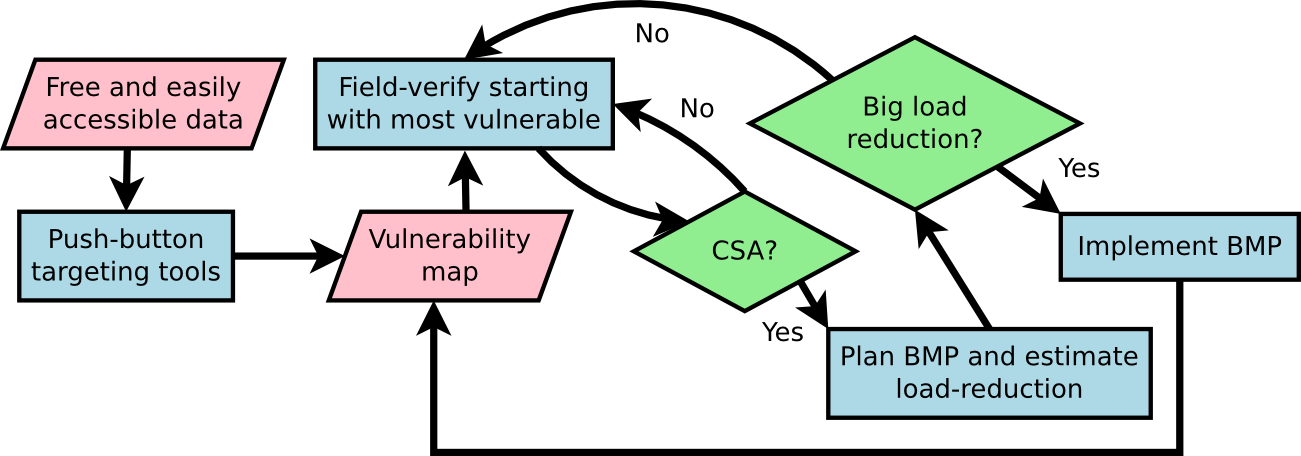
\includegraphics[width=\textwidth]{decisionFramework}
  \caption{Decision framework for identifying Critical Source Areas (CSAs) of non-point source nutrient pollution and prioritizing best management practices (BMPs) on agricultural fields.}
  \label{decisionFramework}
\end{figure}

\section{Methods}
The tools that we have developed are based on a three-variable index. The first variable in the index de-prioritizes agricultural fields if they flow into an internally draining area. These areas are identified using high-resolution Light Detection and Ranging (LiDAR) elevation data with a curve-number-based estimation \cite{aron_infiltration_1977} of runoff for a given precipitation event. The higher spatial resolution of LiDAR elevation data provides a more precise estimation of internally draining areas; prior to widespread LiDAR technology, the only way to make a similar estimation would require using the 10-meter resolution National Elevation Dataset (NED). The coarser resolution of the NED cannot detect small storage pools on the landscape. In many cases, NED does not reflect current human structures, notably road berms, that act as small detention structure for smaller storms. LiDAR solves both of these modeling challenges.

The second variable is the Stream Power Index (SPI), which is a good indicator of gully erosion \cite{galzki_identifying_2011}. Gullies are a more severe form of erosion---that is, they occur when sheet and rill erosion accumulates downslope. Therefore, the presence of gullies can be an indication of large-scale soil and nutrient loss. Fortunately, due to their concentrated nature, the locations of gullies can be identified with some precision using high-resolution elevation data such as LiDAR.

The third variable is a grid-based estimate of soil loss using the Universal Soil Loss Equation (USLE)---the grids required for the estimation are LiDAR elevation data to determine the slope/slope-length factor and the Cropland Data Layer \cite{boryan_monitoring_2011} to determine generalized crop rotations (e.g., dairy or cash grain). The generalized crop rotations are used in a novel methodology for estimating rotational averages of the USLE cover factor. In addition to assessing which fields are vulnerable to erosion, using this methodology we can infer which fields would benefit the most from best management practices, notably tillage type, by performing a sensitivity analysis between traditional tillage and conservation tillage.

\section{Prioritization Results}

The intention of these tools is to target \emph{where} BMP assessment should be prioritized. Therefore, the results are provided as a series of maps. Maps are provided for each of the model components (i.e., internally draining areas, SPI, and soil loss) and all components combined into a composite score. Any of these results can be interpreted at their base resolution (3-meter recommended) or aggregated to the level of an agricultural field (Figure~\ref{fieldScaleTargeting}).

\begin{figure}
  \centering
    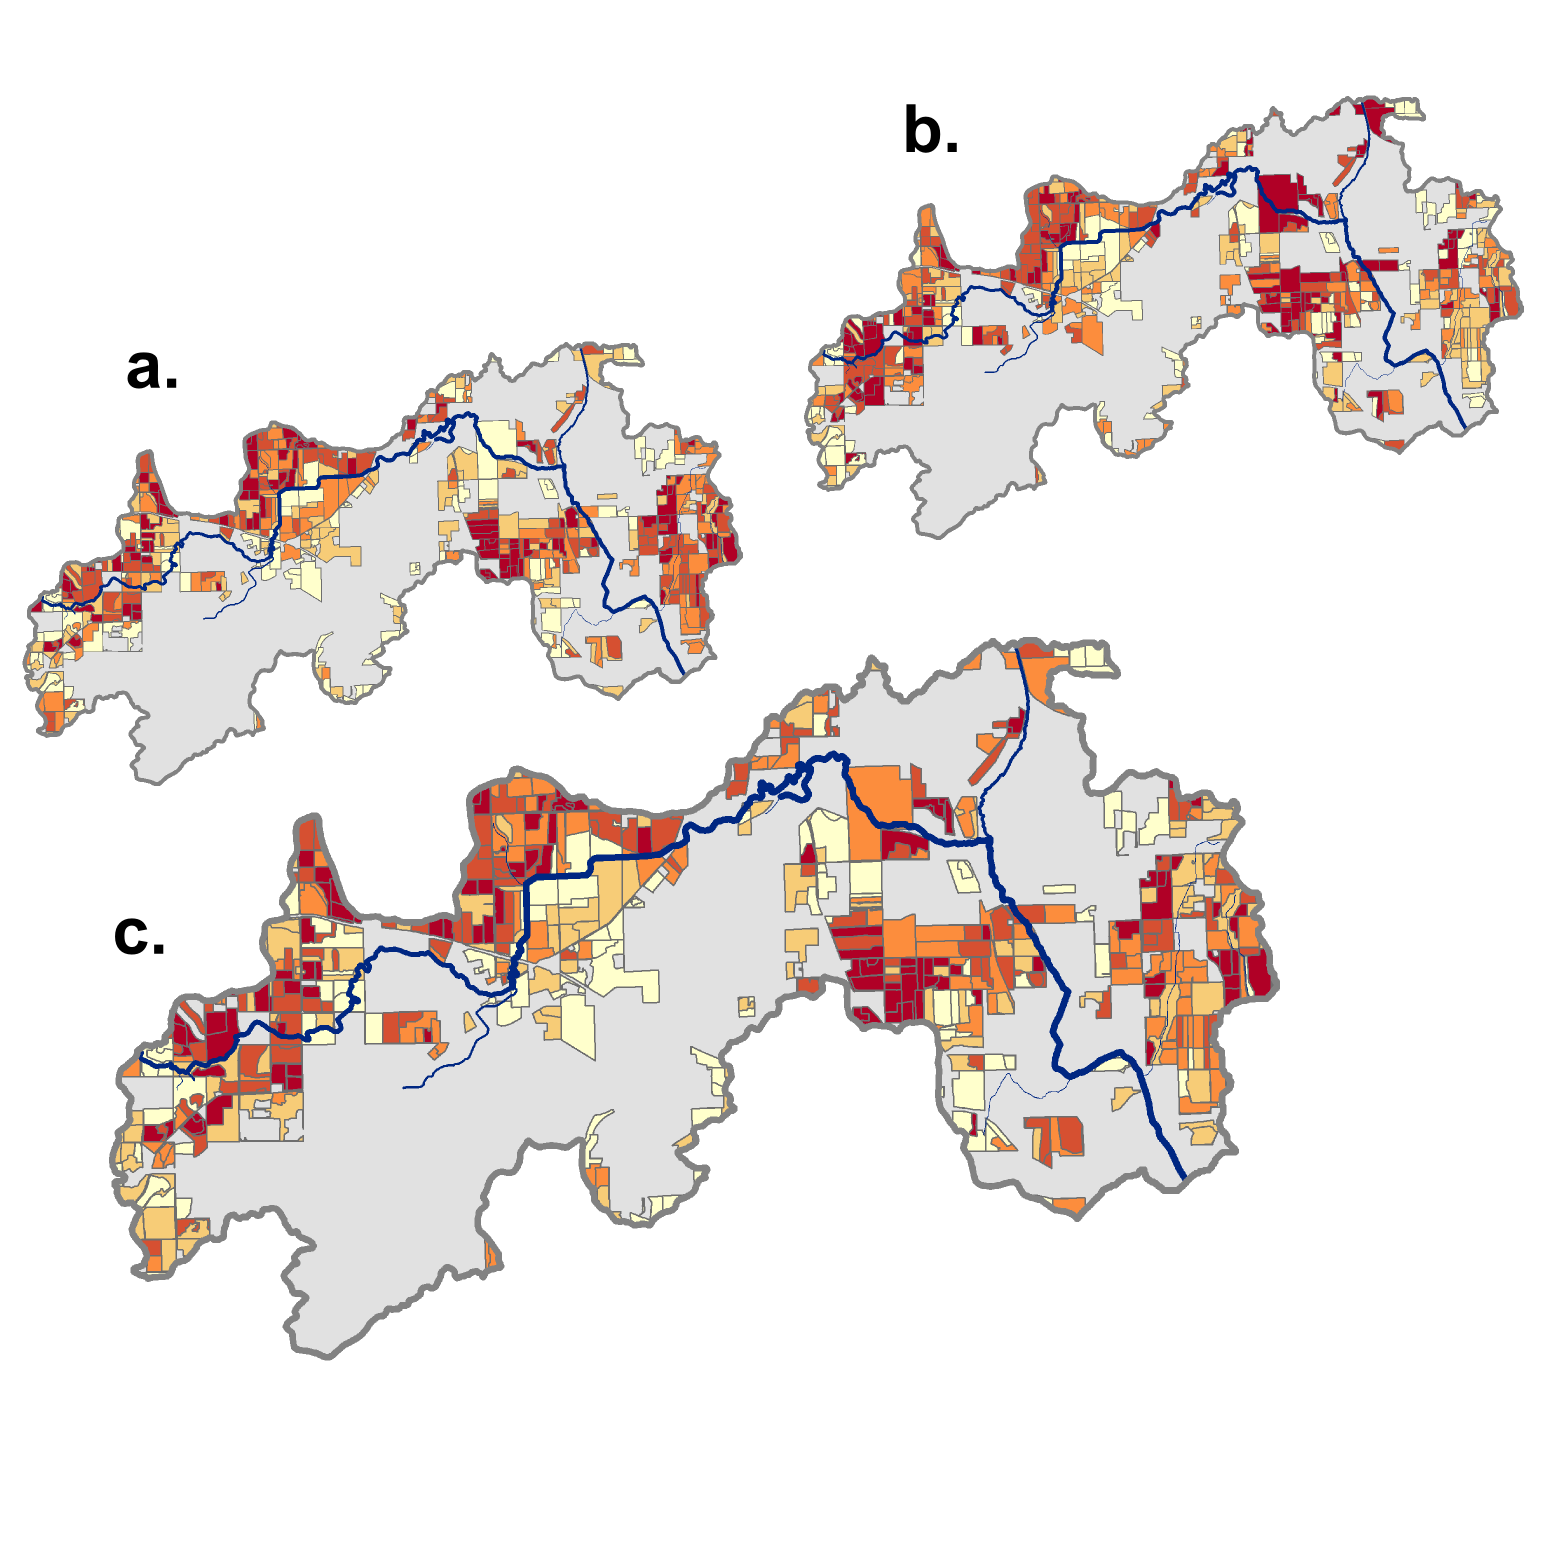
\includegraphics[width=\textwidth]{fieldScaleTargeting}
  \caption{Maps of targeting results aggregated to agricultural fields and ranked by their mean value. Results can be interpreted by input components, such as the Stream Power Index (SPI) (a) or soil loss estimates (b) from the Universal Soil Loss Equation (USLE), or by a composite index (c). Results shown here are low vulnerability (beige) to high vulnerability (deep red).}
  \label{fieldScaleTargeting}
\end{figure}

In addition to the composite results, several intermediate results are provided including, for example, internally draining areas, cover factors, and crop rotations. These individual products can be used to target specific watershed impacts. For example, perhaps it is known that erosion is not the primary pathway for nutrient delivery, however dairy farms have been found to contribute substantially more due to the addition of excessive manure. In this case, perhaps the crop rotational definition can provide additional insight on where to target. Several examples of intermediate layers are shown in Figure~\ref{intermediateLayers}.

\begin{figure}
  \centering
    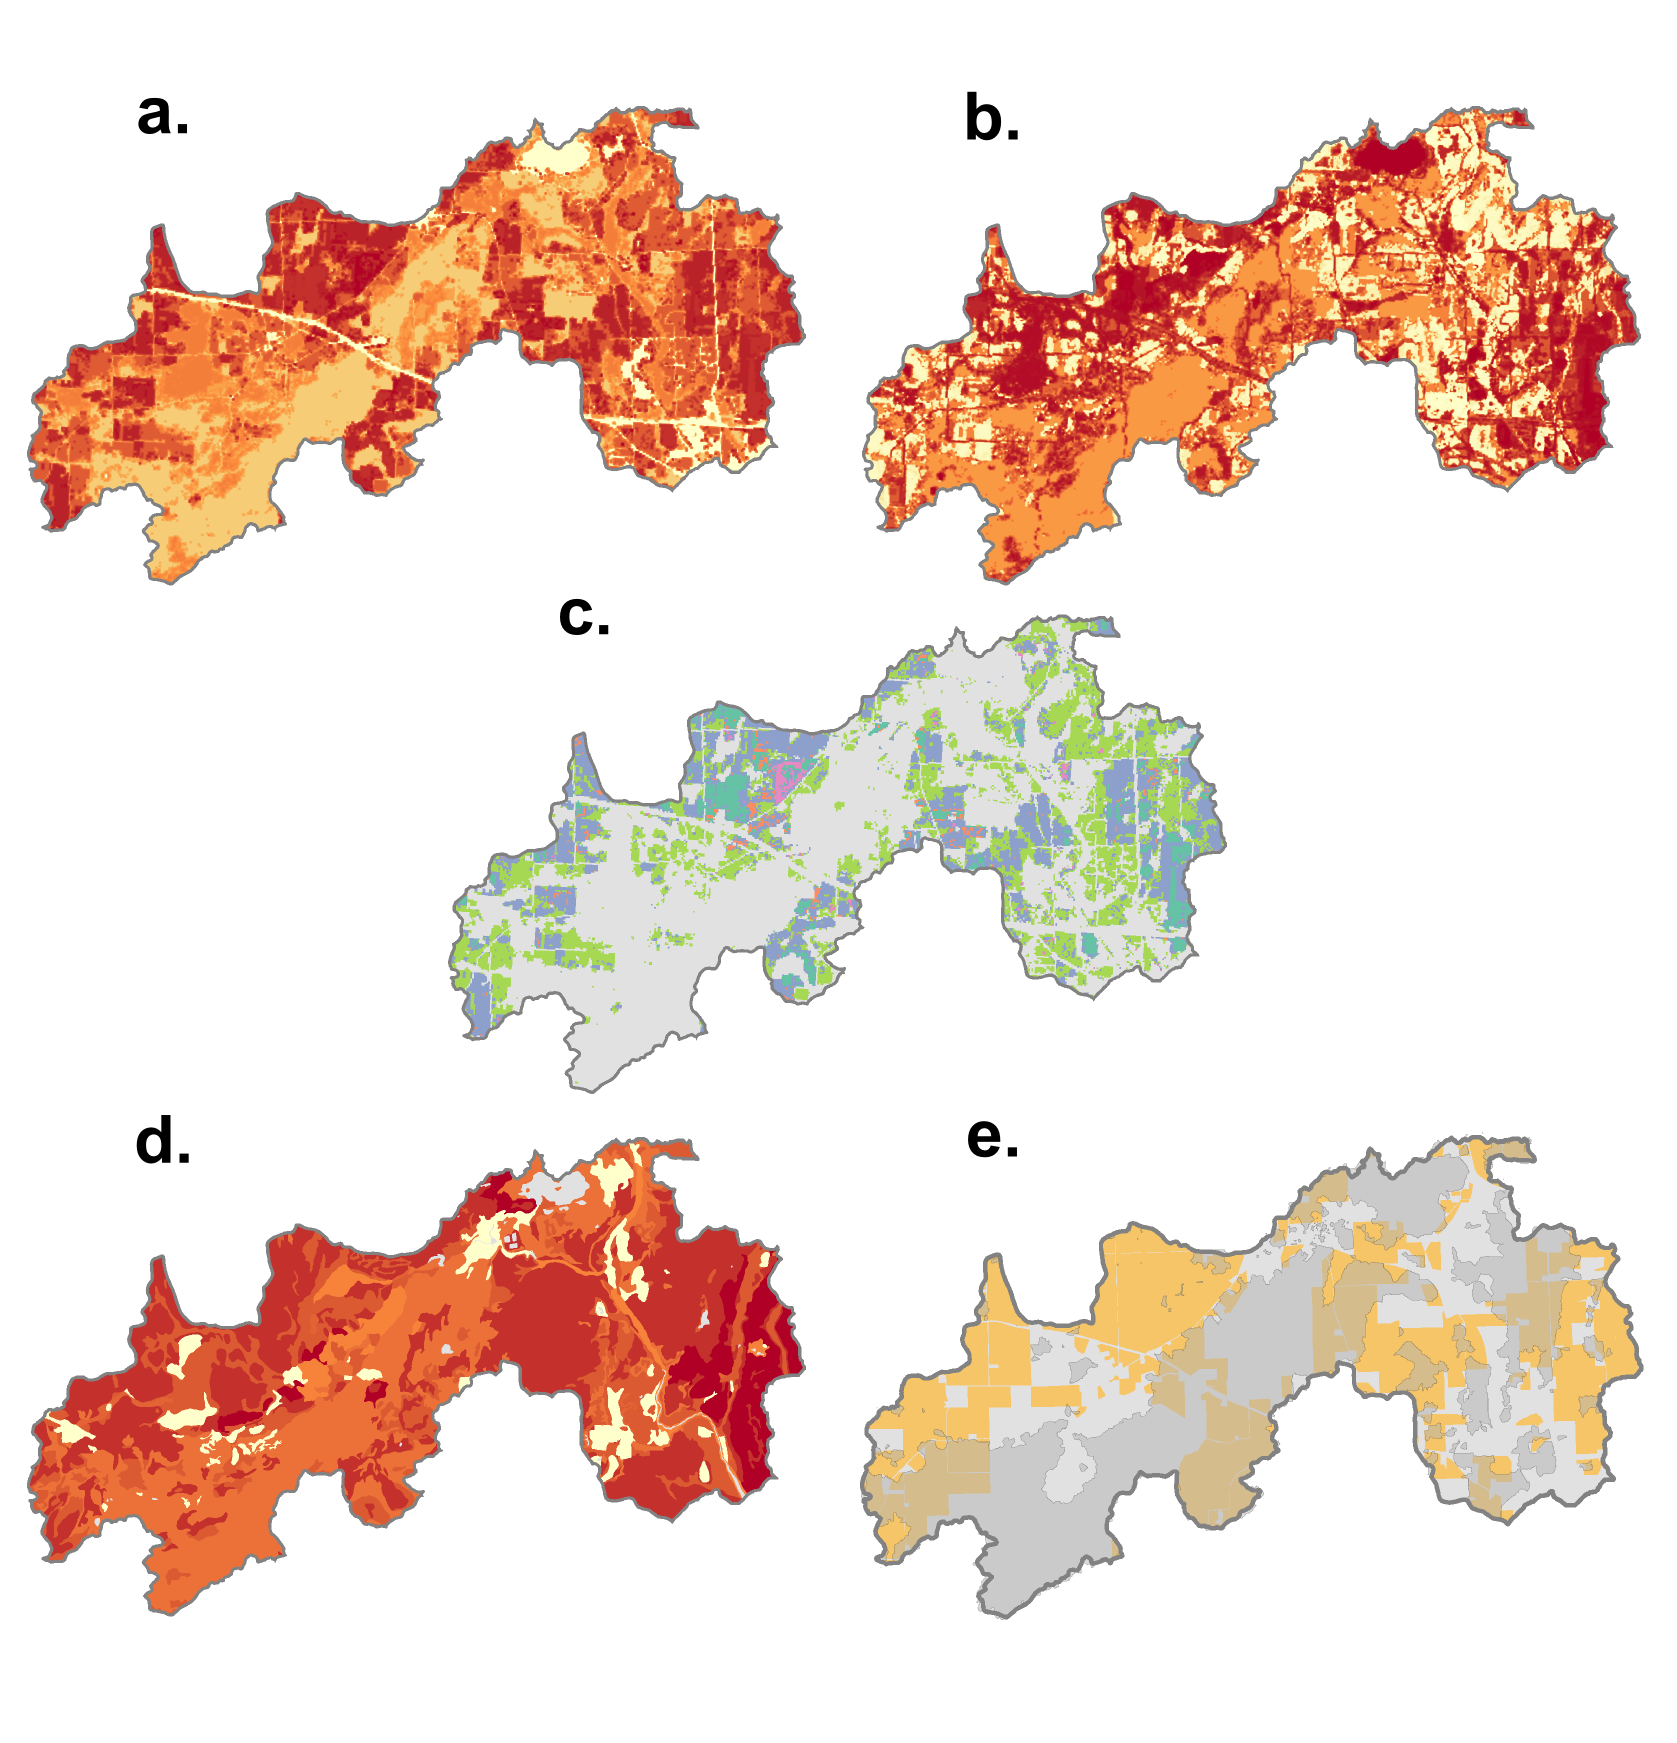
\includegraphics[width=0.89\textwidth]{intermediateLayers}
  \caption{Intermediate layers used to estimate vulnerability. These layers can be used in addition to the vulnerability maps for additional insight. Each map is described from top to bottom: (a) Universal Soil Loss Equation (USLE) cover factor (deep red indicates a significant effect of cropping on erosion); (b) curve number indicating susceptibility to runoff from low (beige) to high (deep red); (c) crop rotation where teal denotes a "cash grain" rotation, orange denotes continuous corn, blue denotes a dairy operation, green denotes pasture or hay, and pink denotes a potato/vegetable rotation; (d) USLE K-factor indication detachable soils from low (beige) to high (deep red); (e) internally drainining areas denoted in dark transparent grey and agriculture in orange---where they overlap are agricultural fields that are estimated to drain internally.}
  \label{intermediateLayers}
\end{figure}

\pagebreak

\bibliography{C:/Users/ruesca/Dropbox/library}
\bibliographystyle{acm}

\end{document}

